\section{Hardware}

\subsection{Drones}

    There are different categories or names for what can be considered a drone, such as UAV (Unmanned Aerial Vehicle), UAS (Unmanned Aerial Systems), RPAS (Remotely Piloted Aircraft System), or Multicopter (Figure \ref{fig:multicopter}). A specific definition is given by the official documentation \cite{ardupilot}, “A multicopter is a mechanically simple aerial vehicle whose motion is controlled by speeding or slowing multiple downward thrusting motor/propeller units.” It is known that each category has distinct functionalities, and therefore, a multicopter is not exactly the same as a UAV. According to the official documentation \cite{ardupilot}, “A multicopter becomes a UAV or Drone when it is capable of autonomous flight.”

    Additionally, according to Piotr et al., "Drones or Unmanned Aerial Systems (UAV - Unmanned Aerial Vehicle or UAS - Unmanned Aerial Systems) are the aircrafts, which are able to fly without a pilot and passengers on board” \cite{piotr_drones}. Another definition comes from The Office of the Secretary of Defense of the United States of America: “A powered, aerial vehicle that does not carry a human operator, uses aerodynamic forces to provide vehicle lift, can fly autonomously or be piloted remotely, can be expendable or recoverable, and can carry a lethal or non-lethal payload.”

    \begin{figure}[h!]
        \centering
        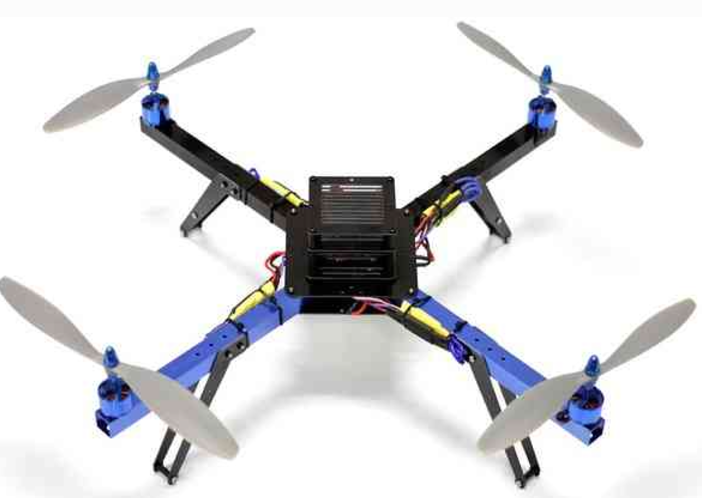
\includegraphics[width=0.6\textwidth]{pictures/multicopter.png}
        \caption{Multicopter.}
        \label{fig:multicopter}
    \end{figure}

    There are various configurations of drones, each with different capabilities and specific applications. Figure \ref{fig:quad_frame} shows the Quad Frame, one of the most common and basic configurations. Quadrotor drones, with four motors and propellers, are ideal for applications like photography, surveillance, and light tasks.

    Figure \ref{fig:hexa_frame} presents the Hexa Frame, with six motors and propellers, offering greater stability and payload capacity. These drones are suitable for tasks requiring the transport of heavier equipment, such as advanced sensors or high-resolution cameras.

    In Figure \ref{fig:octo_frame}, the Octo Frame configuration is shown, featuring eight motors and propellers. Drones with this configuration are ideal for industrial applications due to their higher payload capacity and redundancy, which improves safety in case of motor or propeller failures.

    Finally, Figure \ref{fig:octo_quad_frame} shows the Octo Quad Frame, combining the advantages of eight motors with the efficiency of a compact configuration. These types of drones are used when high payload capacity and precise stability control are required.

    \begin{figure}[h!]
        \centering
        \begin{minipage}[b]{0.4\textwidth}
            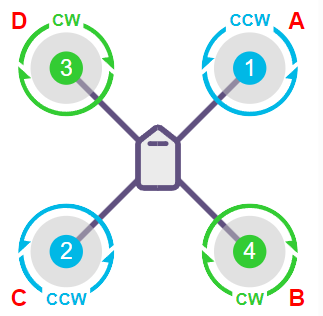
\includegraphics[width=\textwidth]{pictures/quad_frame.png}
            \caption{Quad X Frame.}
            \label{fig:quad_frame}
        \end{minipage}
        \hfill
        \begin{minipage}[b]{0.4\textwidth}
            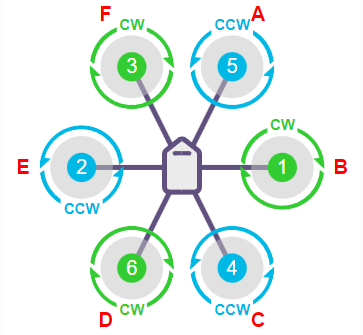
\includegraphics[width=\textwidth]{pictures/hexa_frame.png}
            \caption{Hexa X Frame.}
            \label{fig:hexa_frame}
        \end{minipage}
        \vskip\baselineskip
        \begin{minipage}[b]{0.4\textwidth}
            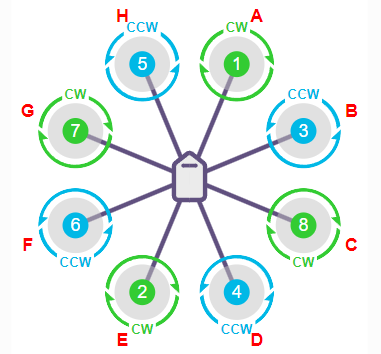
\includegraphics[width=\textwidth]{pictures/octo_frame.png}
            \caption{Octo X Frame.}
            \label{fig:octo_frame}
        \end{minipage}
        \hfill
        \begin{minipage}[b]{0.4\textwidth}
            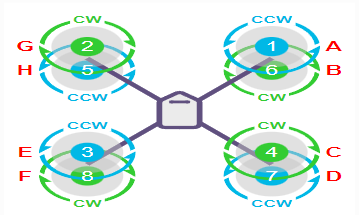
\includegraphics[width=\textwidth]{pictures/octo_quad_frame.png}
            \caption{Octo Quad X Frame.}
            \label{fig:octo_quad_frame}
        \end{minipage}
        \caption{Drone configurations.}
        \label{fig:drone_frames}
    \end{figure}

\subsection{Types of Drone Charging Stations}

    Currently, there is a growing trend towards the concept of charging or docking stations for drones. According to Grlj et al., "A docking station for UAVs is a multipurpose system that enables them to land safely, take off, recharge and/or replace batteries, and transfer data and payload" \cite{grlj_docking_stations}.

    In this context, various types of charging stations can be observed, classified according to the following specifications \cite{grlj_docking_stations}:

    \begin{itemize}
        \item Mobility (fixed and mobile)
        \item Charging method (two electrodes, multiple electrodes, wireless, etc.)
        \item Automatic battery exchange (recharging spare batteries)
        \item Positioning (active and passive)
        \item Drone storage (yes or no)
        \item Package delivery (with storage, without storage)
        \item Type of landing (precision, vision-based, etc.)
        \item Type of landing platform (self-leveling)
    \end{itemize}

    \begin{figure}[h!]
        \centering
        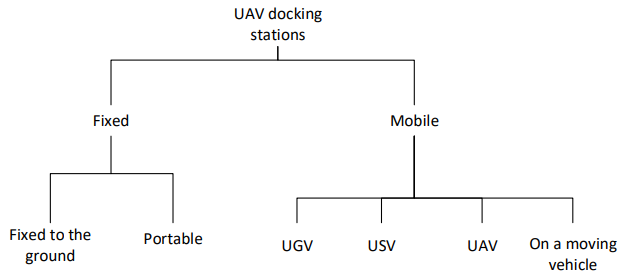
\includegraphics[width=0.7\textwidth]{pictures/charging_classification.png}
        \caption{Drone Charging Stations Classification \cite{grlj_docking_stations}.}
        \label{fig:charging_classification}
    \end{figure}

\subsubsection{Fixed Charging Stations}

    The main objective of fixed charging stations is to provide a stable platform that allows drones to recharge without needing to move the infrastructure during the operation process. These stations are often simpler in design and are placed in strategic locations, such as cities or industrial areas. According to Grlj et al., many of these fixed stations use an active or passive positioning system to ensure the drone lands accurately, and they may feature charging options through electrical contacts or even wireless charging \cite{grlj_docking_stations}.

\subsubsection{Advantages of Fixed Charging Stations}

    Fixed stations are particularly useful in situations where the drone needs a precise landing in a constant location. These stations can use visual markers, such as ArUco [2] markers, to guide the drone during the final landing phase, ensuring high accuracy in the maneuver. Additionally, they may include self-leveling platform systems to guarantee the stability of the drone upon landing, especially on uneven terrain.

    \begin{figure}[h!]
        \centering
        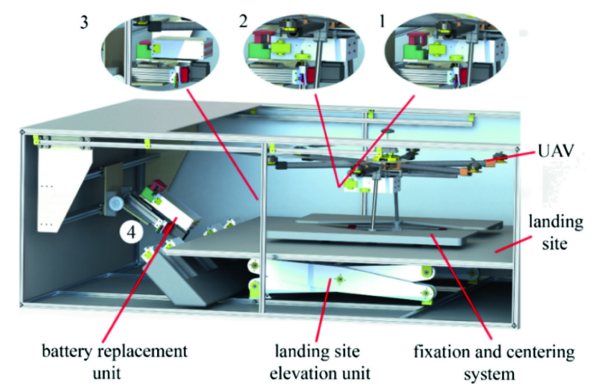
\includegraphics[width=0.6\textwidth]{pictures/fixed_charging_1.png}
        \caption{Fixed docking station with its subsystems. The labels (1–4) show the battery replacement mechanism in operation \cite{grlj_docking_stations}.}
        \label{fig:fixed_charging}
    \end{figure}

    \begin{figure}[h!]
        \centering
        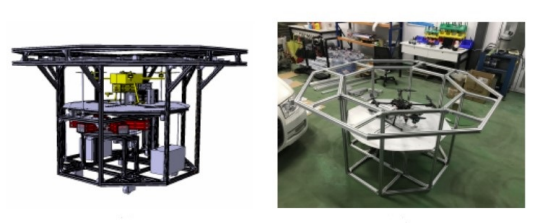
\includegraphics[width=0.6\textwidth]{pictures/fixed_2.png}
        \caption{Battery replacement docking station \cite{grlj_docking_stations}.}
        \label{fig:fixed_charging}
    \end{figure}

    \begin{figure}[h!]
        \centering
        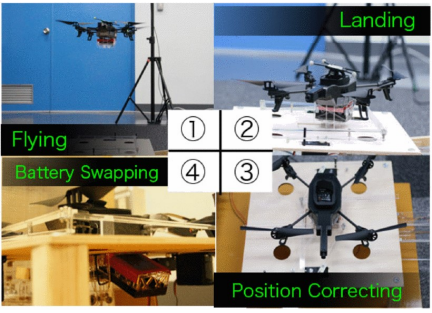
\includegraphics[width=0.6\textwidth]{pictures/fixed_3.png}
        \caption{Endless Flyer \cite{grlj_docking_stations}, docking station with battery replacement mechanism. The labels in the center show the different landing stages and the order in which they are realized.}
        \label{fig:fixed_charging}
    \end{figure}

    \begin{figure}[h!]
        \centering
        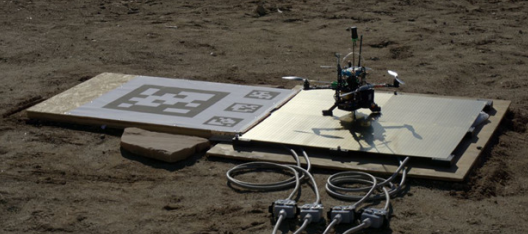
\includegraphics[width=0.6\textwidth]{pictures/fixed_4.png}
        \caption{ Docking station with recharging pad with the custom made UAV from \cite{grlj_docking_stations}. In the figure, the QR codes used in the approach and landing phase can be seen .}
        \label{fig:fixed_charging}
    \end{figure}

\subsubsection{Mobile Charging Stations}

    Mobile charging stations, on the other hand, provide greater operational flexibility, as they are mounted on surface vehicles, such as Unmanned Ground Vehicles (UGVs) or even Unmanned Surface Vehicles (USVs). These stations extend the range of drones by moving to locations that require real-time logistical support, such as in search and rescue operations \cite{grlj_docking_stations}.

\subsubsection{Advantages of Mobile Charging Stations}
    Mobile stations provide a dynamic alternative for supporting drones in missions that require continuous movement. For example, some stations are mounted on autonomous ground vehicles that can move to locations where the drone requires assistance, significantly increasing the operational range of the UAV. These types of stations can also incorporate complex systems to exchange batteries, such as robotic arms that ensure the safe removal and insertion of the drone's battery without needing to pause the mission for long recharge periods.
    
    \begin{figure}[h!]
        \centering
        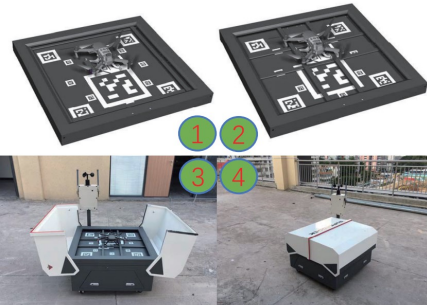
\includegraphics[width=0.4\textwidth]{pictures/mobile_1.png}
        \caption{Moving docking station with storage system and battery replacement system. Labels in the figure (1–4) show the order in which the active positioning mechanism and storing mechanism take place \cite{grlj_docking_stations}.}
        \label{fig:mobile_charging}
    \end{figure}

    \begin{figure}[h!]
        \centering
        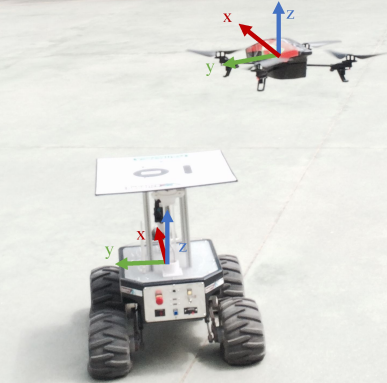
\includegraphics[width=0.4\textwidth]{pictures/mobile_2.png}
        \caption{UGV–UAV proposed moving docking station solution.}
        \label{fig:mobile_charging}
    \end{figure}

    \begin{figure}[h!]
        \centering
        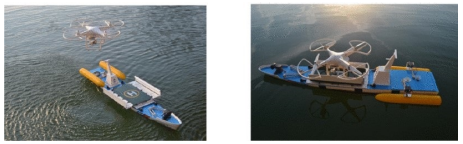
\includegraphics[width=0.6\textwidth]{pictures/mobile_3.png}
        \caption{USV–UAV landing system.}
        \label{fig:mobile_charging}
    \end{figure}


\subsection{Automatic Drawer Mechanism}
    \subsubsection{Types of Mechanisms}
    The automatic drawer mechanism in the charging station for drone storage is similar to the mechanisms found in other automatic storage solutions. Here, we'll discuss the main mechanisms that could be used in this context, including the advantages and disadvantages of each. The mechanism chosen for this project was the belt and V-pulley due to its easy accessibility and low cost.
    
    \paragraph{Pistons} Pistons are a common choice for automated movement in many types of machinery. They use compressed air or hydraulic fluid to extend and retract, making them well-suited for precise and strong movements. For an automatic drawer for drones, pistons could provide a robust and stable means to open and close the drawer. However, this approach may have higher costs and complexity compared to other mechanisms, as it requires pneumatic or hydraulic infrastructure and regular maintenance.
    
    \paragraph{Belt and Toothed Pulley} This mechanism uses a toothed belt and pulley to move the drawer. It offers greater precision compared to V-belts because the toothed design prevents slipping, making it a suitable choice for environments where precise positioning is critical. However, the increased complexity and cost of toothed belts make them less accessible, and they may require more maintenance due to the increased friction between the teeth.
    
    \paragraph{Belt and V-Pulley} This mechanism involves a belt shaped like a V and a pulley, which ensures good friction and prevents slipping while moving the drawer. The belt and V-pulley mechanism is simple, inexpensive, and easy to source, which made it the choice for this project. It offers a balance between precision and accessibility, being a practical solution for the needs of an automatic drone storage drawer. Its main disadvantage is that it may lack the precise positioning capabilities of toothed pulleys, but for the current application, this is acceptable.

    
\subsection{Motors and Propellers}

    \subsubsection{Motors}
    
    Motors are an essential component for the flight of a drone, and they are typically brushless motors due to their high efficiency and durability. According to the guide, the selection of the motor depends on factors such as the drone's size, total weight, and the desired type of flight. Key considerations include:
    
    \begin{itemize}
        \item \textbf{Kv Rating:} Indicates the revolutions per minute (RPM) per applied volt without load. A lower Kv provides more torque, making it ideal for larger drones with bigger propellers.
        \item \textbf{Compatibility:} The motor must be compatible with the electronic speed controller (ESC) and the propellers.
        \item \textbf{Mounting:} The drone's frame design should allow for a secure installation of the motors.
    \end{itemize}
    
    \subsubsection{Propellers}
    
    Propellers generate the necessary lift for flight. According to the guide, they are a critical factor for the drone's performance and should be selected based on the motors and the size of the drone. Important characteristics include:
    
    \begin{itemize}
        \item \textbf{Size (diameter and pitch):} Larger propellers generate more lift but require more powerful motors. The "pitch" determines how much air the propeller displaces per revolution.
        \item \textbf{Material:} Propellers can be made of plastic, wood, or carbon fiber. Carbon fiber propellers are lighter and stronger, making them ideal for high-performance drones.
        \item \textbf{Balancing:} Poorly balanced propellers can cause vibrations, affecting stability and the quality of sensor data.
    \end{itemize}
    
    \subsubsection{LiPo Batteries}
    
    LiPo (Lithium Polymer) batteries are the primary energy source for most drones. They are lightweight, high-capacity, and capable of delivering the current required by the motors and other components. Key aspects include:
    
    \begin{itemize}
        \item \textbf{Cells (S):} Each cell has a nominal voltage of 3.7V. For example, a 3S battery has 11.1V (3 × 3.7V). The number of cells must be compatible with the motors and ESCs.
        \item \textbf{Capacity (mAh):} Determines the flight time. Higher capacity provides longer flights but also increases weight.
        \item \textbf{Discharge Rate (C):} Indicates how much current the battery can safely provide. It must meet the motors' requirements.
        \item \textbf{Charging and Safety:} LiPo batteries require specific chargers and must be handled carefully to prevent fires.
    \end{itemize}
    
    
    
    


